\documentclass[12pt]{article}

% Paquetes básicos para español y acentos
\usepackage[spanish]{babel}
\usepackage[utf8]{inputenc}
\usepackage[T1]{fontenc}
\usepackage{lmodern}

% Paquetes útiles
\usepackage{amsmath, amssymb}
\usepackage{geometry}
\usepackage{setspace}
\usepackage{hyperref}
\usepackage{booktabs}
\usepackage{graphicx}
\usepackage{float}
\usepackage{pgffor}
\usepackage{longtable}


\newcommand{\tablaPNG}[2]{%
    \begin{figure}[H]
        \centering
        \includegraphics[width=0.65\textwidth, keepaspectratio]{#1}
        \caption{#2}
    \end{figure}
}
\geometry{margin=2.5cm}
\onehalfspacing

\title{Data Challenge Airbnb CDMX: ¿En Qué Colonias Conviene Invertir?}
\author{Marco Antonio Torres Salazar, Maximiliano Huitrón Rodríguez\\
Nicole Jiménez Freyermuth, Ramón Sinobas Arencibia }
\date{24 de noviembre de 2025}

\begin{document}

\maketitle
\section{Introducción y pregunta de investigación}

En los últimos años, la Ciudad de México se ha consolidado como uno de los mercados de \textit{Airbnb} más dinámicos de América Latina. La expansión de esta plataforma ha abierto nuevas oportunidades de inversión inmobiliaria, pero también ha vuelto más compleja la decisión sobre \emph{dónde} conviene comprar una propiedad para destinarla a renta de corto plazo. La rentabilidad de un anuncio no depende únicamente del precio por noche, sino también de la ocupación a lo largo del año, de la accesibilidad de la ubicación, de la percepción de seguridad en la zona y de características propias del alojamiento y del anfitrión.

El objetivo de este trabajo es responder a la siguiente pregunta de investigación:

\begin{quote}
\emph{¿Qué colonias de la Ciudad de México ofrecen las mejores oportunidades de inversión en Airbnb, una vez que consideramos simultáneamente precio, ocupación, accesibilidad al transporte y niveles de crimen?}
\end{quote}

Para contestar esta pregunta combinamos tres tipos de información: i) una base detallada de anuncios de Airbnb para la Ciudad de México, ii) estadísticas oficiales de delitos de alto impacto y con perspectiva de género a nivel colonia y alcaldía, y iii) medidas geoespaciales de distancia al transporte público. A partir de estas fuentes construimos dos niveles de análisis:

\begin{enumerate}
  \item \textbf{Modelo a nivel anuncio:} analizamos los determinantes del precio por noche y del ingreso anual estimado de cada anuncio, en función de la distancia al transporte, del crimen en la zona y de características del alojamiento y del anfitrión.
  \item \textbf{Modelo a nivel colonia:} agregamos los anuncios y modelamos el \emph{ingreso anual promedio por colonia} como función del precio promedio, la ocupación promedio, el acceso al transporte, el crimen y efectos fijos de alcaldía. A partir de esta base construimos un \textit{ranking} de colonias desde la perspectiva de inversión.
\end{enumerate}

El análisis se completa con un conjunto de mapas y gráficas descriptivas y con una discusión de limitaciones y posibles extensiones, incluyendo el uso de modelos de lenguaje (LLM) para explotar el texto de las reseñas y construir medidas de satisfacción y percepción de seguridad reportadas por los huéspedes.

\section{Datos y construcción de variables}

\subsection{Fuentes de información}

La primera fuente de datos es el \textit{scraping} de anuncios de Airbnb para la Ciudad de México. Cada observación corresponde a un anuncio individual e incluye variables como el precio publicado por noche (\texttt{price}), las noches mínimas requeridas (\texttt{minimum\_nights}), el número de reseñas recibidas, el número de propiedades administradas por el anfitrión, el tipo de alojamiento (casa/departamento completo, cuarto privado, etc.), la localización geográfica y la alcaldía.

La segunda fuente son los archivos administrativos de delitos de alto impacto y con perspectiva de género. A partir de estos insumos se construyen tasas de delitos por población o por vivienda a nivel colonia y alcaldía. En la base final aparecen variables como la tasa total de delitos de alto impacto (\texttt{alto\_impacto\_total\_tasa}), una medida de \emph{crimen violento} y una medida de delitos especialmente relevantes para turistas.

Finalmente, utilizamos información geoespacial (GTFS y capas de transporte) para calcular la distancia desde cada anuncio al punto de transporte público más cercano (metro, Metrobús, etc.). Esta variable, \texttt{dist\_transporte\_km}, captura la accesibilidad del alojamiento.

\subsection{Variables a nivel anuncio}

Sobre la base de \textit{listings} se realizan varios pasos de limpieza y construcción de variables:

\begin{itemize}
  \item \textbf{Precio en formato numérico.} A partir de la variable original \texttt{price} se elimina el símbolo de peso y las comas, y se convierte a numérico, obteniendo \texttt{price\_num}. Se eliminan observaciones con precio no válido o igual a cero.
  \item \textbf{Trimming de extremos.} Para evitar que unos pocos anuncios atípicos dominen la estimación, se recorta la distribución de precios: se eliminan los anuncios por debajo del percentil 1 y por encima del percentil 99 de \texttt{price\_num}.
  \item \textbf{Logaritmo del precio.} Se construye \(\log(\texttt{price\_num})\), que será la variable dependiente principal en el modelo de precio, lo que permite interpretar los coeficientes como semi-elasticidades.
  \item \textbf{Ocupación e ingreso anual estimado.} A partir de la tasa de ocupación (\texttt{ocupacion\_rate}) se calcula un \emph{ingreso anual estimado} del anuncio:
  \[
  \texttt{ingreso\_anual\_est} \approx \texttt{price\_num} \times \texttt{ocupacion\_rate} \times 365.
  \]
  Esta variable se analiza en niveles y en logaritmos.
  \item \textbf{Variables de crimen.} Para cada anuncio se asignan las tasas de crimen de la colonia o alcaldía en la que se ubica: tasa total de delitos de alto impacto, crimen violento, delitos contra turistas y robo de vehículo. Estas tasas suelen ser pequeñas en niveles, por lo que los coeficientes en las regresiones pueden verse grandes en magnitud, pero la interpretación relevante es el efecto de un cambio razonable en la tasa.
  \item \textbf{Accesibilidad y tipo de alojamiento.} Se incluye la distancia al transporte público más cercano (\texttt{dist\_transporte\_km}) y dummies que indican si el alojamiento es un \emph{entire home} o un \emph{private room}. También usamos el logaritmo del número de reseñas y el número de propiedades administradas por el anfitrión como aproximaciones a reputación y profesionalización del host.
  \item \textbf{Efectos fijos de alcaldía.} Se construye una variable categórica de alcaldía para capturar diferencias sistemáticas entre zonas (por ejemplo, políticas locales, mezcla de usos de suelo, infraestructura) que no observamos directamente.
\end{itemize}

\subsection{Agregación y ranking a nivel colonia}

Con el objetivo de responder directamente a la pregunta de inversión, agregamos la información por colonia y construimos la base \texttt{ranking\_colonias\_inversion}. En esta base cada observación es una colonia y se resumen las variables relevantes:

\begin{itemize}
  \item \texttt{n\_listings}: número de anuncios de Airbnb en la colonia.
  \item \texttt{precio\_promedio}: precio medio por noche entre los anuncios de la colonia.
  \item \texttt{ingreso\_anual\_promedio}: ingreso anual estimado promedio de los anuncios de la colonia.
  \item \texttt{ocupacion\_promedio}: tasa de ocupación promedio.
  \item \texttt{dist\_transporte\_promedio}: distancia promedio al transporte público.
  \item \texttt{tasa\_crimen}: tasa de delitos de alto impacto para la colonia.
  \item \texttt{alcaldia\_geo}: alcaldía a la que pertenece la colonia.
\end{itemize}

En esta base agregada se trabaja principalmente con el logaritmo del ingreso anual promedio (\(\log(\texttt{ingreso\_anual\_promedio})\)) y el logaritmo del precio promedio, además de las variables en nivel de ocupación, distancia y crimen. Esta es la base que usamos tanto para el modelo a nivel colonia como para construir un ranking de colonias desde la perspectiva de inversión.

\section{Análisis descriptivo}

En la base a nivel anuncio contamos con poco más de 20\,000 propiedades activas. El precio por noche tiene una media cercana a \$1{,}450 pesos, con una desviación estándar del orden de \$1{,}500, un mínimo alrededor de \$66 y máximos que superan los \$19{,}000. Esto confirma que el mercado de Airbnb en la ciudad es altamente heterogéneo: coexisten habitaciones muy económicas con propiedades de lujo.

La tasa de ocupación estimada presenta una media aproximada de 0.32 y una desviación estándar de 0.29. Existen anuncios prácticamente desocupados, con tasas cercanas a cero, y otros con ocupaciones casi completas. La combinación de precios muy distintos y ocupaciones muy variables se refleja en una distribución de ingresos anuales extremadamente dispersa.

En términos de ubicación, la distancia al transporte público más cercano es, en promedio, de 0.16 km, con una desviación estándar de 0.15 km, aunque existen propiedades a más de 4 km del transporte. En general, las zonas centrales tienden a concentrar una mayor densidad de anuncios y mejor conectividad, mientras que las periferias combinan mayores distancias con menor densidad de oferta.

Respecto al crimen, las tasas promedio de delitos de alto impacto y delitos violentos son bajas en términos absolutos, pero muestran una variación importante entre colonias y alcaldías. Al cruzar estas tasas con los mapas de precios y ocupación se observan patrones intuitivos: las zonas turísticas y de alta actividad económica suelen tener precios más altos, mejor acceso al transporte y también niveles más elevados de ciertos tipos de delitos.

Al pasar al nivel colonia, la base agregada muestra que algunas colonias concentran un número muy reducido de anuncios, mientras que otras albergan decenas o cientos. El ingreso anual promedio por colonia exhibe diferencias marcadas entre alcaldías: colonias del sur y del poniente con alta demanda turística y residencial generan ingresos anuales promedio considerablemente mayores que colonias periféricas con menor demanda y menor oferta registrada.

\section{Modelos econométricos}

\subsection{Modelo 1: determinantes del precio e ingresos a nivel anuncio}

El primer bloque de modelos utiliza la base a nivel anuncio. La variable dependiente principal es el logaritmo del precio por noche. De manera simplificada, la especificación más completa puede escribirse como:

\begin{align}
\log(\text{precio}_i)
=\, & \alpha 
+ \beta_1 \log(\text{distancia\_transporte}_i) \\
& + \beta_2 \text{tasa\_crimen\_total}_i \\
& + \beta_3 \text{crimen\_violento}_i 
+ \beta_4 \text{crimen\_turista}_i \\
& + \beta_5 \text{robo\_vehiculo}_i \\
& + \gamma^\top X_i
+ \delta_{\text{alcaldía}(i)}
+ \varepsilon_i
\end{align}

donde \(X_i\) incluye características del anuncio (tipo de alojamiento, logaritmo del número de reseñas, número de propiedades del anfitrión, noches mínimas, entre otras) y \(\delta_{\text{alcaldía}(i)}\) son efectos fijos por alcaldía.

Los resultados muestran, de manera consistente, que:

\begin{itemize}
  \item \textbf{Distancia al transporte.} El coeficiente de \(\log(\text{distancia\_transporte})\) es negativo y estadísticamente significativo en todas las especificaciones, con magnitudes alrededor de \(-0.05\) a \(-0.06\). Esto implica que un aumento proporcional en la distancia al transporte se asocia con precios más bajos. Intuitivamente, los anuncios peor conectados tienden a ser más baratos.
  \item \textbf{Crimen.} La tasa de crimen total por sí sola no es robustamente significativa en todas las columnas, pero algunos componentes particulares sí lo son. El crimen violento aparece con un coeficiente positivo y significativo: las zonas con mayor incidencia de delitos violentos tienden a tener precios más altos. Esto no debe interpretarse como que el crimen “eleva” el precio, sino más bien como un reflejo de que áreas céntricas y caras concentran tanto actividad económica como delitos. Por el contrario, los delitos orientados a turistas tienden a asociarse con precios ligeramente menores, lo que es consistente con una posible penalización de zonas percibidas como riesgosas para visitantes.
  \item \textbf{Características del anuncio y del anfitrión.} La especificación más completa incorpora variables como el tipo de alojamiento, el log de reseñas, el número de propiedades del host y las noches mínimas. En general, alojamientos de tipo casa/departamento completo y aquellos con más reseñas tienden a cobrar más por noche, reflejando una mayor disposición a pagar por privacidad y por reputación consolidada. El número de propiedades del anfitrión y las noches mínimas también muestran asociaciones significativas con el precio, sugiriendo que los anfitriones más profesionalizados y las estancias más largas se vinculan con una estrategia de precios distinta.
\end{itemize}

En términos de ajuste, los modelos de precio alcanzan un \(R^2\) de alrededor de 0.25--0.30. Es decir, una fracción importante de la variación en precios se explica por variables observadas de localización, crimen y características del anuncio, pero persiste una parte considerable ligada a atributos no observados (calidad del interior, decoración, servicios específicos, etc.).

Adicionalmente, estimamos modelos donde la variable dependiente es la tasa de ocupación y el logaritmo del ingreso anual estimado. En estos modelos se observa que:

\begin{itemize}
  \item La distancia al transporte no afecta de forma significativa la ocupación, pero sí se asocia negativamente con el ingreso anual, reforzando la idea de que la accesibilidad es clave para la rentabilidad total.
  \item Un precio más alto por noche, manteniendo todo lo demás constante, está asociado con menores ingresos anuales. Esto refleja el trade-off entre precio y ocupación: incrementos en el precio pueden reducir la demanda lo suficiente como para disminuir el ingreso anual total.
  \item Las variables de reputación (número de reseñas) y el tipo de alojamiento se relacionan positivamente tanto con la ocupación como con el ingreso anual.
\end{itemize}

En conjunto, el modelo a nivel anuncio nos permite entender qué características micro de la propiedad y del entorno se traducen en precios más altos y en ingresos anuales mayores.

\subsubsection*{Diccionario de Variables Modelo 1}

\paragraph{Variables Dependientes}
\subparagraph{log\_price}
Logaritmo natural del precio por noche: $\log(\text{price} + 1)$. Normaliza la distribución y permite interpretar cambios porcentuales.

\subparagraph{ocupacion\_rate}
\[
\text{ocupacion\_rate} = \frac{365 - \text{availability\_365}}{365}
\]
Proporción de días ocupados; proxy directo de demanda.

\subparagraph{ingreso\_anual\_est}
\[
\text{ingreso\_anual\_est} = \text{price} \times (365 - \text{availability\_365})
\]

\subparagraph{log\_ingreso\_anual}
\[
\log(\text{ingreso\_anual\_est} + 1)
\]
Transformación logarítmica que facilita interpretación y reduce asimetrías.

\paragraph{Variables Independientes Principales}
Incluye:
\begin{itemize}
    \item log\_dist\_transporte\_m: logaritmo de la distancia al transporte más cercano (signo esperado negativo).
    \item alto\_impacto\_total\_tasa: tasa de criminalidad relativa.
    \item delito\_violento: delitos violentos de alto impacto.
    \item delito\_turista: delitos que afectan directamente al visitante.
\end{itemize}

\paragraph{Controles}
\begin{itemize}
    \item entire\_home y private\_room (tipo de alojamiento),
    \item log\_reviews, log\_reviews\_ltm (reputación),
    \item calculated\_host\_listings\_count (número de propiedades del host),
    \item minimum\_nights (mínimo de noches).
\end{itemize}

\paragraph{Interacción}
\textbf{dist\_x\_delito}: interacción entre distancia y crimen para evaluar complementariedad o sustitución.

\paragraph{Efectos Fijos}
\textbf{alcaldia\_geo}: controla heterogeneidad no observable por alcaldía.

\paragraph{Variables para el Ranking}
score\_precio, score\_ocupacion, score\_seguridad, score\_transporte y score\_total.

\paragraph{Resumen de signos esperados}
Distancia y crimen negativos; entire\_home y private\_room positivos; minimum\_nights ambiguo.

\subsection{Modelo 2: ingreso anual promedio a nivel colonia}

El segundo bloque de análisis se realiza sobre la base agregada por colonia. La variable dependiente es el logaritmo del \emph{ingreso anual promedio} de los anuncios localizados en cada colonia. La especificación general es:

\begin{align}
\log(\text{ingreso\_anual\_promedio}_c)
=\, & \alpha
+ \beta_1 \log(\text{precio\_promedio}_c) \\
& + \beta_2 \text{ocupacion\_promedio}_c \\
& + \beta_3 \text{dist\_transporte\_promedio}_c \\
& + \beta_4 \text{tasa\_crimen}_c \\
& + \beta_5 \big(\text{dist\_transporte\_promedio}_c 
\times 
\text{tasa\_crimen}_c\big) \\
& + \delta_{\text{alcaldía}(c)}
+ u_c.
\end{align}

Estimamos cuatro especificaciones:

\begin{enumerate}
  \item \textbf{Modelo básico:} sólo incluye el log del precio promedio y la ocupación promedio.
  \item \textbf{Modelo con transporte y crimen:} añade la distancia promedio al transporte y la tasa de crimen.
  \item \textbf{Modelo con interacción:} añade la interacción entre distancia y crimen, para capturar si el efecto del crimen depende de qué tan accesible es la colonia.
  \item \textbf{Modelo con efectos fijos de alcaldía:} replica la tercera especificación e incorpora efectos fijos por alcaldía.
\end{enumerate}

Los resultados muestran patrones muy claros:

\begin{itemize}
  \item \textbf{Precio y ocupación promedio.} Tanto el logaritmo del precio promedio como la ocupación promedio son altamente significativos en todas las especificaciones. Los coeficientes de \(\log(\text{precio\_promedio})\) están cercanos a 1, lo que sugiere que un aumento de 1\% en el precio promedio se traduce, aproximadamente, en un aumento de 1\% en el ingreso anual promedio de la colonia, manteniendo constante la ocupación. Por su parte, los coeficientes de ocupación promedio rondan 3.4, de modo que un aumento de 0.1 puntos en la ocupación (por ejemplo, de 0.3 a 0.4) se asocia con un incremento de alrededor de 0.34 puntos logarítmicos en el ingreso anual, es decir, en torno a 40\%.
  \item \textbf{Transporte y crimen.} Ni la distancia promedio al transporte ni la tasa de crimen resultan estadísticamente significativas una vez que controlamos por precio y ocupación. La interacción entre ambas tampoco es significativa. Esto sugiere que el impacto de la accesibilidad y del crimen sobre la rentabilidad de la colonia ya está incorporado en los niveles de precio y ocupación: colonias menos accesibles o con más crimen tienden a tener menores precios y/o ocupaciones, y estos canales son los que realmente importan para el ingreso anual promedio.
  \item \textbf{Efectos fijos de alcaldía.} Al introducir efectos fijos por alcaldía, el \(R^2\) del modelo aumenta de aproximadamente 0.847 a 0.858. Algunos coeficientes de alcaldía resultan significativamente negativos (por ejemplo, Iztapalapa, Azcapotzalco, Cuajimalpa, Tlalpan o La Magdalena Contreras), lo que indica que, incluso controlando por precio, ocupación, transporte y crimen, las colonias de estas alcaldías tienden a generar ingresos anuales promedio menores que la alcaldía de referencia. Otras alcaldías, como Cuauhtémoc o Benito Juárez, no difieren significativamente de la referencia, lo que sugiere que las diferencias dentro de estas alcaldías se explican principalmente por variación intra-alcaldía en precio y ocupación.
\end{itemize}

En conjunto, los modelos a nivel colonia presentan un muy buen ajuste (con \(R^2\) superiores a 0.84) y confirman que, para evaluar la conveniencia de inversión, lo más relevante es combinar el nivel de precios con la ocupación efectiva, más que enfocarse de forma aislada en el crimen o en la accesibilidad.

\subsubsection*{Diccionario de Variables Modelo 2}

\paragraph{Objetivo del Modelo}
Este modelo explica el ingreso anual promedio por colonia considerando: precio promedio, ocupación promedio, distancia al transporte, criminalidad y efectos fijos por alcaldía.

\paragraph{Variable Dependiente: log\_ingreso\_prom}
\[
\text{log\_ingreso\_prom} = \log(\text{ingreso\_anual\_promedio})
\]
El ingreso anual se calcula por anuncio como:
\[
\text{ingreso\_anual\_est} = \text{price} \times (365 - \text{availability\_365})
\]
y posteriormente se promedia por colonia. El uso de logaritmo reduce asimetría y facilita interpretación porcentual.

\paragraph{Variables Independientes Principales}

\subparagraph{log\_precio\_prom}
Coeficiente positivo, cercano a 1, altamente significativo en todas las especificaciones. Colonias con mayor precio promedio generan ingresos sustancialmente mayores.

\subparagraph{ocupacion\_promedio}
Proporción de días ocupados en la colonia. Coeficiente grande (3.37–3.41) y muy significativo: la ocupación es tan determinante como el precio para explicar ingresos.

\subparagraph{dist\_transporte\_promedio}
Mide accesibilidad. El signo esperado es negativo, pero en los modelos no resulta significativo una vez que se controla por precio, ocupación y alcaldía.

\subparagraph{tasa\_crimen}
Proporción de delitos de alto impacto de la colonia respecto al total de CDMX. No muestra efectos significativos sobre el ingreso anual promedio.

\subparagraph{Interacción dist\_transporte\_promedio $\times$ tasa\_crimen}
Explora si la combinación inseguridad–distancia afecta el ingreso. El coeficiente no es significativo en ninguna especificación.

\paragraph{Efectos Fijos por Alcaldía (factor(alcaldia\_geo))}
Capturan diferencias no observables entre alcaldías: prestigio, servicios, calidad urbana, historia y regulación. Mejoran el ajuste del modelo (R\textsuperscript{2} pasa a 0.858).

\paragraph{Resumen de Resultados}
\begin{itemize}
    \item Precio y ocupación son los determinantes más robustos.
    \item Transporte y crimen no presentan efectos significativos.
    \item Las diferencias entre alcaldías explican variación territorial importante.
\end{itemize}

\paragraph{Especificaciones del Modelo}
\begin{itemize}
    \item \textbf{Modelo básico:} precio y ocupación (R\textsuperscript{2} = 0.846).
    \item \textbf{+ Transporte y crimen:} poco aporte adicional.
    \item \textbf{+ Interacción:} sin evidencia robusta.
    \item \textbf{+ FE alcaldía:} mejora sustancial del ajuste.
\end{itemize}

\section{Resultados y ranking de colonias}

Con la base \texttt{ranking\_colonias\_inversion} y los resultados del modelo a nivel colonia construimos un \textit{ranking} de colonias desde la perspectiva de inversión. El criterio central es el \emph{ingreso anual promedio} de los anuncios en cada colonia, considerando también la cantidad de anuncios disponibles y la estabilidad de la ocupación.

Las primeras posiciones del ranking están ocupadas por colonias que combinan tres características:

\begin{enumerate}
  \item \textbf{Precios por noche relativamente altos}, típicos de zonas con buena oferta de servicios, cercanía a puntos de interés y demanda turística consolidada.
  \item \textbf{Tasas de ocupación elevadas}, que garantizan que el precio alto realmente se traduzca en ingresos anuales y no en anuncios caros pero vacíos.
  \item \textbf{Buena accesibilidad y niveles de crimen manejables}, que influyen indirectamente sobre precio y ocupación.
\end{enumerate}

En el top del ranking aparecen colonias de distintas alcaldías, incluyendo zonas del sur (como Lomas de San Bernabé en La Magdalena Contreras, Estadio Olímpico en Coyoacán o Rincón del Pedregal en Tlalpan) y colonias más céntricas con alta conectividad. Esta diversidad muestra que no existe una única “alcaldía ganadora”, sino combinaciones específicas de colonia y entorno.

Desde la perspectiva de un inversionista, el ranking permite identificar tres perfiles de colonia:

\begin{itemize}
  \item \textbf{Colonias premium de alta rentabilidad:} alto precio y alta ocupación, generalmente bien conectadas y con amplia oferta de servicios. Son candidatas naturales para inversión, aunque suelen requerir una inversión inicial elevada.
  \item \textbf{Colonias de oportunidad:} precios todavía moderados pero con buena ocupación y potencial de apreciación. Suelen estar relativamente cerca de zonas premium y pueden beneficiarse de procesos de consolidación turística o residencial.
  \item \textbf{Colonias de alto riesgo:} niveles de ingreso anual promedio bajos, ya sea por precios reducidos, por ocupaciones bajas o por ambas. En muchos casos se ubican en alcaldías con efectos fijos negativos y mayores niveles de vulnerabilidad social.
\end{itemize}

El ranking no debe leerse como una recomendación automática, sino como una herramienta para priorizar el análisis de colonias en las que la combinación de precio y ocupación ya está generando flujos de ingresos atractivos.

\section{Limitaciones y extensiones (LLM y sentimientos)}

Aunque los resultados son informativos, el análisis tiene varias limitaciones:

\begin{itemize}
  \item \textbf{Causalidad vs. correlación.} Los modelos son esencialmente correlacionales. No podemos afirmar que el crimen “cause” cambios en precio o en ocupación; es plausible que la causalidad corra en ambas direcciones o que exista un factor común (como la centralidad urbana) que aumente simultáneamente la actividad económica y la incidencia delictiva.
  \item \textbf{Medición del crimen.} Las tasas de delito se basan en registros administrativos que pueden estar sujetos a subreporte y errores de georreferenciación. Además, la variable relevante para la decisión de los huéspedes es la \emph{percepción} de inseguridad, que no siempre coincide con los datos oficiales.
  \item \textbf{Foto en un momento del tiempo.} El análisis es estático: utiliza un corte temporal específico y no captura estacionalidad, shocks temporales (por ejemplo, eventos masivos) ni cambios estructurales en el mercado de Airbnb o en la seguridad de la ciudad.
  \item \textbf{Variables omitidas.} No observamos directamente la calidad interior de los alojamientos, la decoración, servicios específicos (vista panorámica, gimnasio, alberca), ni la estrategia de precios dinámica de los anfitriones. Estos factores pueden explicar parte de la variación remanente en precios e ingresos.
\end{itemize}

Una extensión natural del proyecto es explotar de manera sistemática el texto de las reseñas utilizando modelos de lenguaje (LLM). De hecho, construimos un script en \texttt{Python} que, a partir del texto de cada comentario, asigna calificaciones de 1 a 5 en distintas dimensiones (valoración general, limpieza, comunicación, ubicación, relación calidad-precio y sensación de seguridad). Con una submuestra de reseñas ya procesadas es posible:

\begin{itemize}
  \item Construir índices de \textbf{satisfacción promedio} y de \textbf{percepción de seguridad} por anuncio y por colonia.
  \item Incorporar estos índices a los modelos de precio e ingreso como nuevas variables explicativas, para evaluar si las zonas con mejores evaluaciones subjetivas generan rendimientos superiores.
  \item Analizar discrepancias entre seguridad “objetiva” (tasas de crimen) y seguridad “percibida” en las reseñas, y su efecto sobre la demanda.
\end{itemize}

Por restricciones de tiempo y de cómputo (el número total de reseñas es muy grande), el componente de LLM se deja principalmente como línea de trabajo futuro, pero abre una vía interesante para enriquecer la medición de calidad y riesgo desde la perspectiva de los huéspedes.

\section{Conclusiones y recomendaciones para inversionistas}

Este trabajo combina información de Airbnb, estadísticas de crimen y datos geoespaciales de transporte para evaluar la conveniencia de invertir en propiedades destinadas a renta de corto plazo en la Ciudad de México. A partir de un modelo a nivel anuncio identificamos los factores que explican los precios por noche y los ingresos anuales de cada propiedad, y con un modelo a nivel colonia construimos un ranking de zonas desde la perspectiva de inversión.

Los principales mensajes pueden resumirse en tres puntos:

\begin{enumerate}
  \item \textbf{Precio y ocupación son los determinantes centrales de la rentabilidad.} Tanto a nivel anuncio como a nivel colonia, el ingreso anual está dominado por la combinación de precio por noche y tasa de ocupación. Variables como la accesibilidad al transporte y el crimen importan principalmente en la medida en que afectan esas dos dimensiones.
  \item \textbf{La localización importa, pero de forma matizada.} Estar cerca del transporte público se asocia con mayores precios e ingresos, mientras que el crimen presenta una relación ambigua: algunas zonas céntricas y caras tienen más delitos reportados, por lo que el signo de los coeficientes no debe interpretarse de forma ingenua. Es más útil pensar en el conjunto de atributos de la colonia (centralidad, servicios, percepción de seguridad) que en una sola variable.
  \item \textbf{Existen colonias claramente más atractivas que otras.} El ranking construido muestra que ciertas colonias, distribuidas en varias alcaldías, concentran anuncios con ingresos anuales promedio muy altos. Estas colonias combinan buena conectividad, demanda turística o residencial fuerte y una oferta de alojamientos profesionalizada.
  Sobre las dummies de alcaldía, los coeficientes negativos (como los que aparecen para Iztapalapa, Azcapotzalco, Cuajimalpa, Tlalpan y, en menor medida, La Magdalena Contreras) nos dicen que, a igualdad de precio promedio, ocupación, distancia a transporte y tasa de crimen, las colonias ubicadas en esas alcaldías generan menos ingreso anual promedio que las colonias de la alcaldía base. Es decir, hay un “descuento estructural” asociado al territorio: incluso si encuentras una colonia de Iztapalapa con buen nivel de ocupación y un precio razonable, en promedio sigue rindiendo menos que una colonia equivalente en la alcaldía base. En cambio, alcaldías como Cuauhtémoc, Miguel Hidalgo, Benito Juárez o Coyoacán no muestran coeficientes significativamente distintos de cero, lo que sugiere que, una vez controlados los fundamentales, no penalizan sistemáticamente el ingreso anual; ahí el desempeño depende mucho más de las características específicas de la colonia (precio, ocupación, cercanía a transporte, etc.) que de la alcaldía en sí.
Combinando el modelo a nivel anuncio (precio y ocupación explicados por crimen, transporte y tipo de propiedad) con el modelo agregado por colonia (log\_ingreso\_prom) y el ranking de colonias para inversión, la conclusión para un inversionista es clara: las mejores oportunidades están en colonias que combinan precios por noche relativamente altos, alta ocupación, buena accesibilidad al transporte y que además se ubican en alcaldías sin penalización estructural (como Cuauhtémoc, Miguel Hidalgo, Benito Juárez o Coyoacán). Ahí, el modelo muestra que cada 1\% adicional en precio y cada aumento en ocupación se traducen casi uno a uno en más ingreso anual. En contraste, colonias de alcaldías con coeficientes negativos (como Iztapalapa, Azcapotzalco o Tlalpan) tienden a ser menos atractivas desde la perspectiva de renta turística: para compensar ese “descuento territorial” habría que comprar muy barato o asumir una rentabilidad esperada más baja. En resumen, dados los dos modelos y el ranking construido, la estrategia natural es priorizar colonias en alcaldías centrales y relativamente consolidadas, con alta ocupación y buen nivel de precios, y evitar —salvo ganga muy clara— las colonias de alcaldías con efecto fijo negativo importante.

\end{enumerate}

Para un inversionista, las recomendaciones prácticas son:

\begin{itemize}
  \item Utilizar el ranking de colonias como punto de partida para filtrar zonas, priorizando aquellas con ingresos anuales promedio altos y un número suficiente de anuncios como para que la estimación sea estable.
  \item Dentro de las colonias mejor posicionadas, enfocarse en propiedades que mantengan un equilibrio razonable entre precio y ocupación esperada. Subir mucho el precio sin cuidar la ocupación puede reducir el ingreso total.
  \item Considerar el perfil de riesgo: inversionistas más aversos al riesgo pueden preferir colonias del top del ranking con tasas de crimen bajas y buena conectividad, mientras que inversionistas dispuestos a asumir más riesgo pueden explorar colonias con alto potencial de apreciación donde la demanda está creciendo pero los precios aún no se han ajustado completamente.
\end{itemize}

Finalmente, el uso de modelos de lenguaje para analizar reseñas ofrece una vía prometedora para afinar tanto el ranking como las recomendaciones individualizadas. Integrar métricas de satisfacción, de percepción de seguridad y de calidad del servicio permitiría construir, en trabajos futuros, un sistema más completo de evaluación de oportunidades de inversión en el mercado de Airbnb en la Ciudad de México.

Aquí presentamos el ranking de colonias con el mayor potencial de inversión en Airbnb.

\begin{figure}[H]
    \centering
    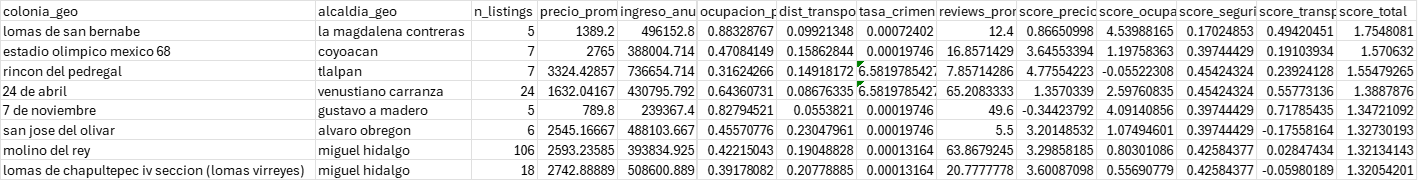
\includegraphics[width=1\textwidth]{output/mejores_colonias.png}
    \caption{Ranking de las mejores colonias para invertir en Airbnb}
    \label{fig:mejores_colonias}
\end{figure}

\section{Figuras}

\foreach \image/\captiontext in {
    boxplot_distancia_por_alcaldia.png/Distribución de distancias al transporte por alcaldía,
    histograma_distancia_transporte.png/Histograma de distancias al transporte público,
    mapa_airbnb_y_transporte.png/Mapa de concentraciones Airbnb y red de transporte público,
    mapa_alto_impacto_homicidio_doloso_2025.png/Homicidio doloso por colonia (2025),
    mapa_alto_impacto_robo_a_transportista_con_y_sin_violencia_2025.png/Robo a transportista con y sin violencia (2025),
    mapa_concentracion_airbnb_colonias_AZUL.png/Concentración de Airbnb por colonia (color azul),
    mapa_concentracion_airbnb_colonias_negro.png/Concentración de Airbnb por colonia (color negro),
    mapa_delitos_genero_total_2025.png/Delitos con perspectiva de género (2025),
    mapa_delitos_total_2025.png/Delitos totales por colonia (2025),
    mapa_precio_airbnb_colonias.png/Mapa de precios de Airbnb por colonia,
    mapa_transporte_publico.png/Mapa de transporte público y zonas Airbnb,
    precio_vs_distancia_transporte.png/Relación entre precio de Airbnb y distancia al transporte público
}{
    \begin{figure}[H]
        \centering
        \includegraphics[width=0.95\textwidth]{figs/\image}
        \caption{\captiontext}
        \label{fig:\image}
    \end{figure}
    \clearpage
}

\section{Tablas}

\begin{center}
\vspace*{\fill}
\tablaPNG{output/tablas_regresion/tabla0_descriptivas.png}{Cuadro 1. Estadísticas descriptivas}
\vspace*{\fill}
\end{center}

\tablaPNG{output/tablas_regresion/tabla1_precio.png}{Cuadro 2. Determinantes del Precio de Airbnb en CDMX}

\tablaPNG{output/tablas_regresion/tabla3_ocupacion_ingresos.png}{Cuadro 3. Ocupación e Ingresos Anuales Estimados}

\tablaPNG{output/tablas_regresiones2/modelo_colonias_ingreso.png}{Cuadro 4. Modelo por colonia: Ingreso estimado}

\end{document}
